\chapter{Sharing Immutable Data}

So far, we have been concerned with the wasteful overhead that results from
a data representation. But what about the data itself? If you examine any Java
heap, you will find that a
large amount of the data is duplicated. At one extreme, 
there are often thousands of copies of the same boxed
integers, especially 0 and 1. At the other extreme, there may be many
 small data
structures that have the same shape and data. 
And, of course, duplicate strings are extremely common.
This chapter describes various
techniques for sharing data to avoid
duplication, including a few low-level mechanisms that Java provides.

\section{String Literals}
\label{sec:literals}

Duplicate strings are not only one of the
most common sources of memory waste, they are also very expensive, since even
small strings incur a large overhead. Fortunately, it is not
hard to eliminate string duplication. 

 One technique is to represent strings as static 
literals whenever possible. A duplication problem arises when dynamically
 created strings
are stored in the heap without any check to see if they already
exist. String literals are stored in a
\emph{string constant pool} when classes
are loaded, where they can be shared.  

 As an example, suppose an application
reads in property name-value pairs from files into tables:
\begin{shortlisting}
class ConfigurationProperties {
    ..
	void handleNextEntry() {
		String propertyName = getNextString();
		String propertyValue = getNextString();
		propertyMap.put(propertyName, propertyValue);
	}
}
\end{shortlisting}
The strings stored in \code{propertyMap} are all created dynamically. If 
there are just a few distinct property names in all of the input pairs, these
property names will be duplicated many times in the heap.

However, if you know in advance what all of the property names are, then you can
define them as static strings, which can be shared among the
entries of \code{propertyMap}.
\begin{shortlisting}
class PropertyNames {
	public static String numberOfUnits = ``NUM_UNITS'';
	public static String minWidgets = ``MIN_WIDGETS'';
	..
}

class ConfigurationWithStaticProperties {
    void handleNextEntry() {
       String propertyName = getNextPropertyName(); 
       String propertyValue = getNextString();
       propertyMap.put(propertyName, propertyValue);
    }
}
\end{shortlisting}
The \code{getNextPropertyName} method reads in a property name, and returns
a pointer to a property name literal. The
property name literal strings themselves
 are stored once in the string constant pool,
not in the heap. Alternatively, instead of using string literals, 
an enumeration type of property names may be a better stylistic choice.

A common
 mistake is to create a new string unnecessarily. For example, in the
following code, there is no need to create new strings from literals.
\begin{shortlisting}
class PropertyNames {
	public static String numberOfUnits = 
	                           new String(``NUM_UNITS'');
	public static String minWidgets = 
	                           new String(``MIN_WIDGETS'');
	..
}
\end{shortlisting}
Even though the standard library is smart enough not to share the
character arrays in this case, this code still creates redundant \code{String}
objects in the heap.

Using static strings to eliminate dulication is only possible when the string
values are known in advance. 
Section~\ref{sec:sharing-pools} introduces the notion of a sharing pool for
sharing dynamic data. Section~\ref{sec:sharing-strings} describes the Java
string interning mechanism, which uses a built-in string sharing pool to
eliminate duplication.

\section{Sharing Pools}
\label{sec:sharing-pools}

Suppose an application generates a lot of duplicated data and the values
are unknown before execution. 
You can eliminate data duplication by using a \emph{sharing pool}, as shown
in Figure~\ref{fig:sharing-pool}. In Figure~\ref{fig:sharing-pool}(a), objects
A and B point to identical data structures.
Figure~\ref{fig:sharing-pool}(b) shows objects A and B sharing the same data
structure, which is stored in a sharing pool.
 \begin{figure}
  \centering
 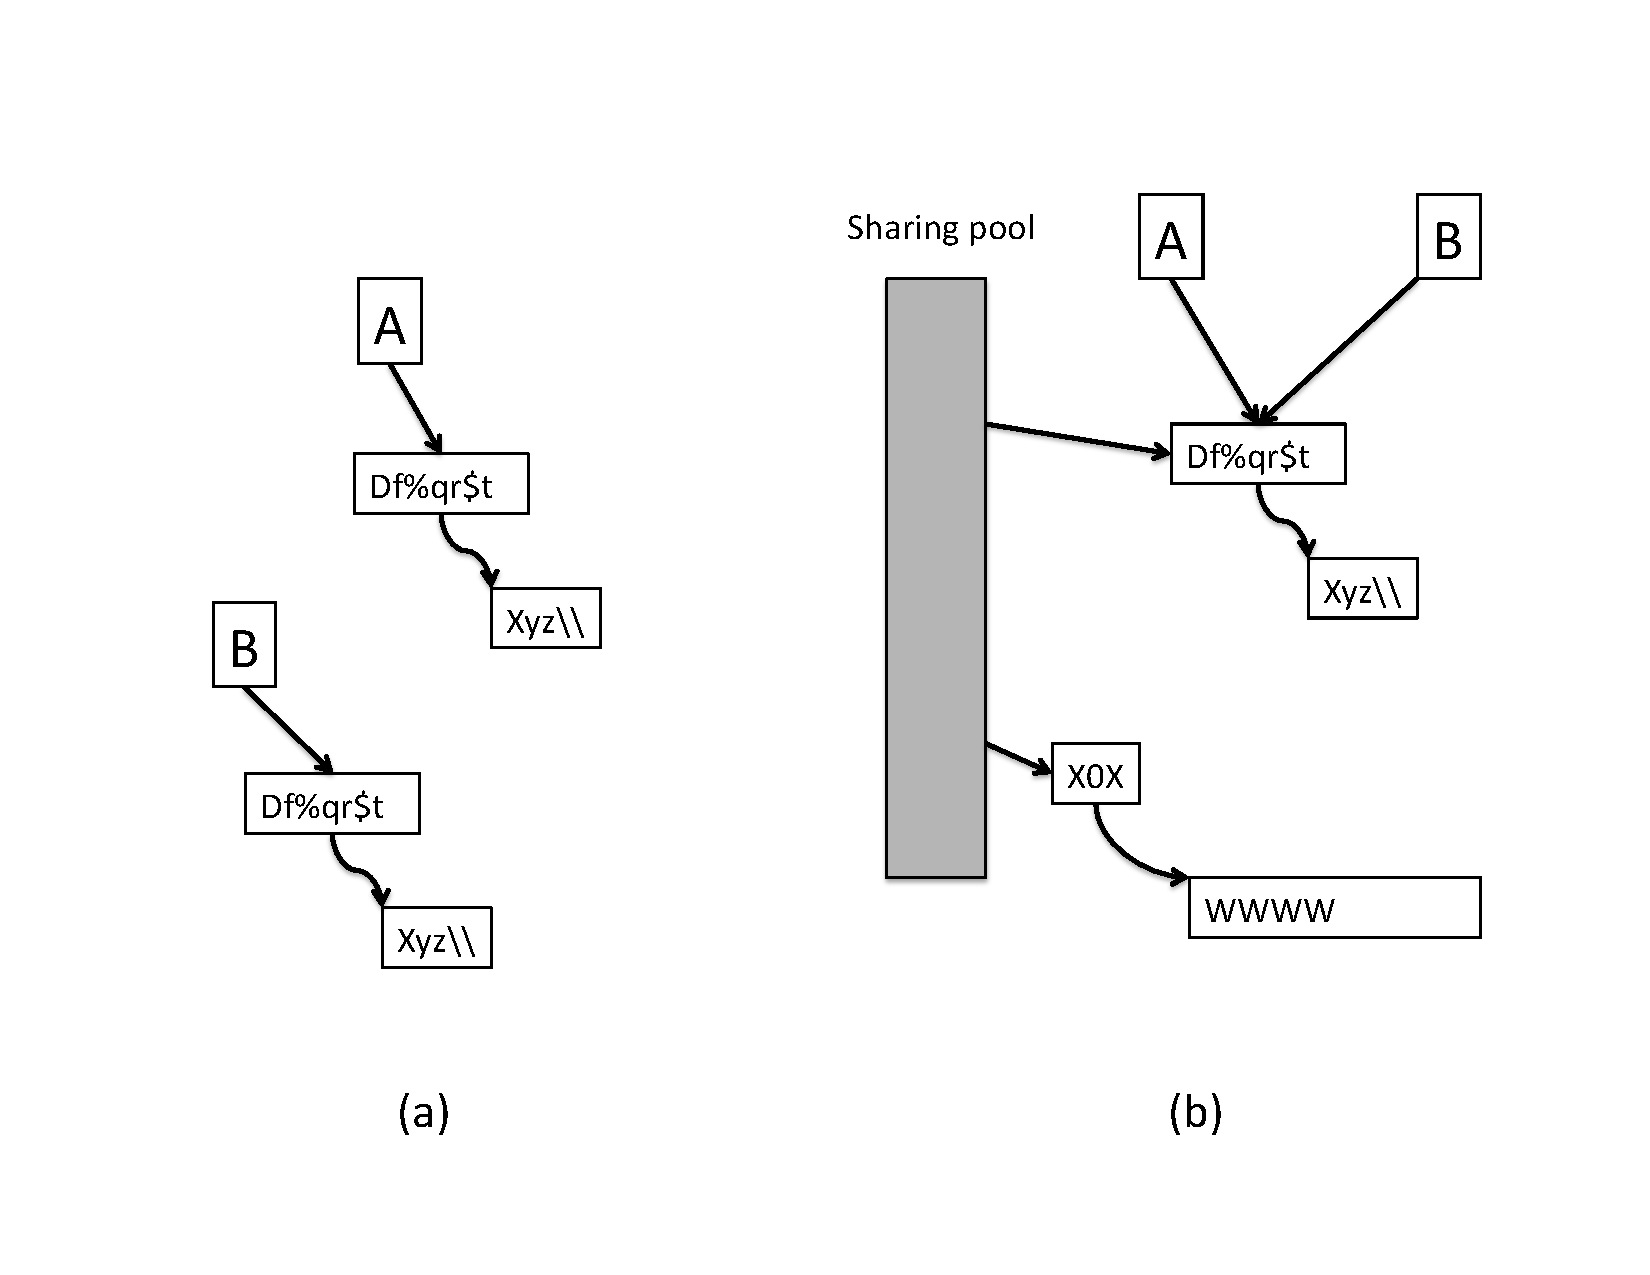
\includegraphics[width=.80\textwidth]{part2/Figures/chapter4/sharing-pool.pdf}
  \caption{(a) Objects A and B point to duplicate data. (b) Objects A and B
  share the same data, stored in a sharing pool.}
  \label{fig:sharing-pool}
\end{figure}

\callout{callout:sharing-pool}{Sharing Pool}{
A \emph{sharing pool} is a centralized structure that stores 
canonical data values that would otherwise be replicated in many objects.
A sharing pool itself is usually some sort of hash table, although it
could be implemented in other ways.
}

There are several issues that you need to be aware of before using a sharing
pool.
\paragraph{Shared objects must be immutable.} Changing shared data can
have unintended side effects. For example, 
changing A in Figure~\ref{fig:sharing-pool}(b), 
also changes the value of B.

\paragraph{Sharing objects changes identity semantics.} 
The result of equality testing should be the same, whether or
not objects are shared.
 In particular, you should never use == on shared objects.
In Figure~\ref{fig:sharing-pool}, \code{A==B} is false in
Figure~\ref{fig:sharing-pool}(a) and true in Figure~\ref{fig:sharing-pool}(b),
 which can lead to very subtle bugs. It is a bad idea to use == in any case,
 unless exact object identity is really required.
 
\paragraph{Sharing pools should not be used if there is limited sharing.}
A sharing pool itself adds
memory costs, including additional per-entry costs. If there is not
much sharing, then the memory saved from
eliminating duplicates isn't enough to compensate for the
extra cost, and memory is being wasted instead of saved. 

\paragraph{Shared objects should be garbage collected.}
In Figure~\ref{fig:sharing-pool}(b), the sharing pool stores an object
that no other object is pointing to. Over time, the sharing pool can fill up
with garbage, that is, items that were once needed but not any more. If the
sharing pool is not purged of these unused items, there is a memory
leak that can eventually use up all of memory.

Fortunately, Java provides a few built in mechanisms that make sharing data
straightforward, and take care of some of these concerns.

\section{String Interning}
\label{sec:sharing-strings}

%Before storing a 
%To use a sharing pool, before storing a new
%\class{String}, first check the pool to see if it is already there. If it is,
%reuse it; otherwise, add the new string to the pool. 
%One catch is that if you end up adding many strings to
%the pool that are never reused, then you will waste memory, since the pool
%structure itself has overhead. So you need to have a good idea
%which strings are likely to have duplicate values.

 Since string duplication is so common, Java provides a built-in string pool
 for sharing \class{String}s, implemented by the native JVM and maintained in
 its internal \emph{perm space}. To share a \class{String}, you simply call the
 method \code{intern} on it, and everything is taken care of automatically.
Since strings are immutable, sharing is safe. However, the rule about not
using == on shared strings still holds.
  
In the example from section~\ref{literals},
\class{ConfigurationWithStaticProperties} eliminates property
name duplication but not
property value duplication. Suppose you know that there are
not too many distinct values, but you don't know what they are. Property
values are perfect candidates for interning.
\begin{shortlisting}
 
 class ConfigurationPropertiesWithInterning {
    void handleNextEntry() {
       PropertyName propertyName = getNextPropertyName(); 
       String propertyValue = getNextString().intern();
       propertyMap.put(propertyName, propertyValue);
    }
}
\end{shortlisting}

The call to \code{intern} will add the new property value string
 to the internal string
pool if it isn't there already, and return a pointer to it. Otherwise, the
new string is a duplicate, and a previously saved string is returned.

Even though interned strings are not stored in the heap, they do incur native
memory overhead, and native memory is not free.
 Interning strings indiscriminately wastes memory and can result in an
 exception: \code{java.lang.OutOfMemoryError:PermGen Space}. 
There are JVM parameters to adjust the perm space size:
XX:PermSize=128m sets perm size to 128 megabytes, and -XX:MaxPermSize=512m sets
the maximum perm size to 512 megabytes. Fortunately, the JVM performs garbage
collection on the internal string pool, so there is no danger of a memory leak.

 %    * Literal strings within the same class in the same package represent
%     references to the same String object. * Literal strings within different
 %    classes in the same package represent references to the same String
%     object. * Literal strings within different classes in different packages
 %    likewise represent references to the same String object. * Strings
 %    computed by constant expressions are computed at compile time and then
   %  treated as if they were literals. * Strings computed by concatenation at
    % run time are newly created and therefore distinct.
\section{Integer Sharing Pool}

The Java library provides a sharing pool for \class{Integer}s. 
Unlike the string pool, the \class{Integer} pool is initialized at class load
time to store all \class{Integer}s in a fixed range, from -128 to 127 by
default. The method \code{Integer.valueOf(int value)} returns a pointer to an \class{Integer} 
in the pool, provided \code{value} is in range.

Because the \class{Integer} sharing pool is pre-initialized and fixed in size,
it's always a good idea to call \code{Integer.valueOf} instead of the constructor to
create a new \class{Integer}. For example, the following code stores
\class{Integer}s from 1 to 500 in an array:
\begin{shortlisting}
    for (int i = 1; i <= 500; i++) {
        numbers[i] = Integer.valueOf(i);
    }
\end{shortlisting}
For the first 127 numbers, \code{valueOf} returns an existing \class{Integer}. 
For the rest of the numbers, \code{valueOf} returns a new
\class{Integer}.  Calling \class{Integer.valueOf} incurs no extra overhead,
and you never have to worry about wasting memory or getting a
memory exception. The only precaution is avoid using == to compare potentially
shared \class{Integer}s.

There is a JVM parameter to change the size of the \class{Integer} sharing pool:
-XX:AutoBoxCacheMax=100 sets the high value in the pool to 100.

\section{Sharing Objects}

Beyond strings and boxed \class{Integer}s, there are often other kinds of
duplicated objects and data structures consuming large portions of the heap. 
There is no built-in Java mechanism to share objects or data
structures in general, so you have to implement a sharing pool from scratch.
All of the sharing pool issues from Section~\ref{sec:sharing-pools} need to be
addressed. The shared objects or structures must be immutable, they must not be
compared using ==, there must be sufficient memory savings from sharing to
justify the sharing pool, and the sharing pool must be not cause a memory leak. 
Note that, in general, \code{equals} is
implemented as ==, so sharing data structures typically requires writing a new
\code{equals} method.

To illustrate a user-written sharing pool, consider a graph where the nodes
have annotations, many of which are duplicates. Both the graph and the
annotations are modified dynamically. The two basic requirements are 1) the
ability to find existing annotations quickly to share them, and 2) the ability
to release annotations that are no longer associated with any node, so they can
be garbage collected.  The second requirement prevents a memory leak. 

Interestingly, none of the common collection classes meet these
requirements out-of-the-box. A \class{HashSet}\<Annotation\> stores
\class{Annotation}s uniquely, but retrieving an existing \class{Annotation} is not easy. 
The first requirement is best implemented as a \class{HashMap} mapping
\class{Annotation}s to themselves:
\begin{shortlisting}
 	HashMap<Annotation><Annotation>   (1)
\end{shortlisting}

For the second requirement, Java provides some support for releasing unused
items from collections, namely, \class{WeakReference}s and \class{WeakHashMap}s. 
A \class{WeakReference} is an object wrapper. An object that is referenced by
a \class{WeakReference} can be reclaimed by the garbage
collector if there are no other strong references to it. A \class{WeakHashMap}
is a hashmap that stores keys as \class{WeakReferences}. That is, when there are no
strong references to a key, the entire entry is freed for garbage collection. 
 For example, we want an \class{Annotation} to
go away when its associated \class{Node}s are no longer used.
This can be implemented by a \class{WeakHashMap}:
\begin{shortlisting}
   WeakHashMap<Node><Annotation> nodeAnnotations;        (2)
\end{shortlisting}

This looks close to what we need. So let's modify (1) to be a
\class{WeakHashMap}, so that when an \class{Annotation} is no longer used,
 its sharing pool entry is freed for
garbage collection:
\begin{shortlisting}
   WeakHashMap<Annotation><Annotation> sharingPool;     
\end{shortlisting}
This should do it. Wrong! Both the key and the value of the sharingPool
 reference the same \class{Annotation} object. The key is a
weak reference, but the value is a strong reference, which prevents an
\class{Annotation} object from every being released. The value must also be a
\class{WeakReference}. Here is the correct
implementation of a sharing pool for \class{Annnotation}s:
\begin{shortlisting}
class AnnotationFactory {
   static WeakHashMap<Annotation, WeakReference<Annotation>>sharingPool = 
                   new WeakHashMap<Annotation, WeakReference<Annotation>>();
    
    public Annotation getAnnotation(Annotation annotation) {
        if (annotation == null) return null;
        WeakReference<Annotation> wref = sharingPool.get(annotation);
        if (wref != null) {
            Annotation oldAnnotation = wref.get();
            if (oldAnnotation != null) {
                return oldAnnotation;
            }
        }
        sharingPool.put(annotation, new WeakReference(annotation));
        return annotation;
    }
    ..
}
\end{shortlisting}

As this example shows,  Java's weak referencing capability has subtle
semantics and is not easy to use. Weak referencing is a lifetime management
facility, and is discussed in greater detail in Chapter~\ref{??} .

\section{Using The Right Container}

Analysis of what�s wrong with this example.
So this was an example from one of the Lotus frameworks, from Sametime Gateway, and this 
was one piece of a session connection, and like all the other examples, it�s one piece of a 
data puzzle with other problems and other sources of costs. It was kind of a medium scale run. 
We saw that the biggest part of this data structure had sessions 110 of them. Each of them had 2 
StringBuffers, and that was taking the bulk of the space here.  We looked in to it, and they had 
quite a few different problems. We saw these StringBuffers sitting in the long lived heap, and 
thought, why would anyone store stringbuffers as permanent memory. Typically stringbuffers are 
used as temporaries. They have very aggressive storage allocation, kind of like the collectio
ns, 
with the thought in mind that you are going to grow them. You are going to be editing them.  
Typically, long-lived memory doesn�t have that problem. Typically, Strings in particular, you 
build them up, and then they are pretty stable. So it seems sort of strange. Usually 
StringBuffer
 is 40\% empty space, because it has a doubling algorithm for allocating them.
 The other strange thing was that they had 3 of them per session, and then there was the 
 question of whether they needed them at all. Turns out we looked at the code, and they had a 
 confluence of 3 different issues going on here. First of all, they had a somewhat delegated 
 design, and again, this was one of the consequences that delegated designs can have, where it 
 causes coding pattern to be duplicated. So in this case, for a completely different reason, 
 they had taken their session objects and split them into 3 parts. And they had some good design 
 reasons for doing that for some replication functionality they needed. But along with that, 
 they took a coding pattern that said that everytime they call toString on this thing for some 
 logging purpose, we�re going to save the contents of that String so that we don�t have to 
 recomputed it. That was really their main problem, that they didn�t realize how much space 
 they were 
taking 
up by saving this computation. And sometimes that�s indeed worth it. 
That you compute something and hold onto it.  In this case they realized they didn�t need to hold 
onto that much stuff. So in this case they had 3 problems. One is they were holding onto it, 
and it got multiplied by 3 because it was a delegated design. The second problem was they were 
holding onto it, and they may not need to. The third problem was they were going to hold onto it,
 
StringBuffer was the wrong thing to use.  In the end, they would have been better off 
trimming the StringBuffer, or just calling toString on it, and getting a shorter 
String out of it.



The JVM stores string literals in a \emph{string constant pool}. Since strings
are immutable, it is safe for the JVM to eliminate duplicates, and keep just
one copy of each literal string. In the following code, the JVM stores two
strings, \code{``Harry''} and \code{``Tom''} in the constant pool, and
\code{name1} and \code{name3} share the string \code{``Harry''}.
\begin{shortlisting}
class BunchOfStrings {
	String name1 = ``Harry'';
	String name2 = ``Tom'';
	String name3 = ``Harry'';
}
\end{shortlisting}

 

